\documentclass{beamer}

\usetheme{Madrid}
\usepackage[english]{babel}
\usepackage[utf8]{inputenc}
\usepackage{times}
\usepackage[T1]{fontenc}
\usepackage[labelfont=bf]{caption}
\usepackage[font=small,labelfont=bf]{subcaption}

%% For figures numbered by section
\usepackage{chngcntr}
\counterwithin{figure}{section}
\counterwithin{table}{section}

%% For bookmarks
\usepackage{bookmark} 

%% Bibliography
\usepackage[backend=bibtex,
natbib=true, 
style=chicago-authordate]{biblatex}
\addbibresource{Returns.bib}
\def\bibfont{\small}

%% For color in text
\usepackage{xcolor}

%% For sparklines in table
\usepackage{graphicx} 
\usepackage{lmodern} 
\newcommand{\graph}[3]{
	\raisebox{-#1mm}{\includegraphics[height=#2em,width=3cm]{#3}}
}

%% For tables in panel
\usepackage{ltablex,ragged2e}
\renewcommand\tabularxcolumn[1]{>{\RaggedLeft}p{#1}}

%% For own made graphs
\usepackage{tikz}

\usepackage{relsize}
\usepackage{tabularx}
\usepackage{tabulary}
\usepackage{multirow}

\title[Depreciation and Returns to Education] 
{Can Depreciation of Human Capital Explain Recent Trends in the Returns to Education?}
\author{Suhas D. Parandekar}
\date[WB Workshop, 2020]{Returns to Education World Bank Workshop, 2020}

\begin{document}
	
%%%%%%%%%%	
\begin{frame}
	\titlepage
\end{frame}

%%%%%%%%%%	
\begin{frame}{Outline}
	\tableofcontents
\end{frame}
	
%%%%%%%%%%
\section{Motivation}
	\subsection{Stylized facts about Human Capital in the Russian Federation}

%%%%%%%%%%
\begin{frame}{Motivation}{Human Capital Levels and Growth Rates: 2001-2014}
\begin{center}
\begin{columns}	
\begin{column}{.6\linewidth}
	\centering
	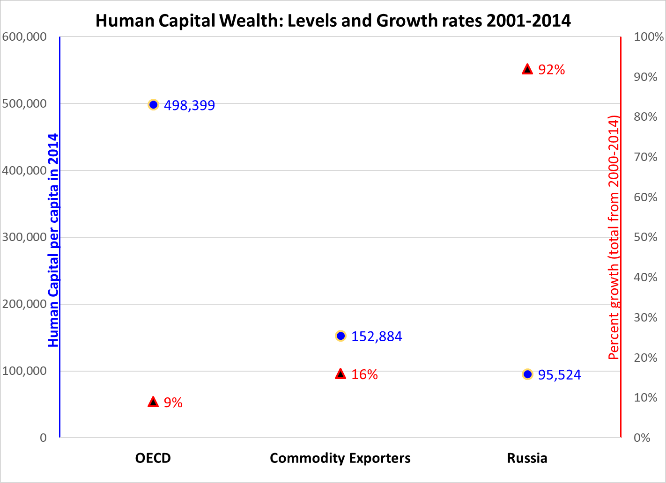
\includegraphics[]{graph_1a.png}
\end{column}
\begin{column}{.4\linewidth}
     \begin{itemize}
        	\item
           	Per capita HC:
        	\begin{itemize}
         		\item OECD - 500,000\$
          		\item Russia -  95,000\$
          	\end{itemize}
          	\item
          	With the 2000-2010 level of HC growth (4.7\%), it would take \textasciitilde 50 years to catch up with the OECD
     \end{itemize}
\end{column}
\end{columns}
\end{center}
\end{frame}

%%%%%%%%%%
\begin{frame}{Motivation}{Peak in Enrollment in University Education (HSE Yearbook)}
\begin{figure}
	\centering
	\vspace*{-0.2in}
	\hspace*{-0.3in}
	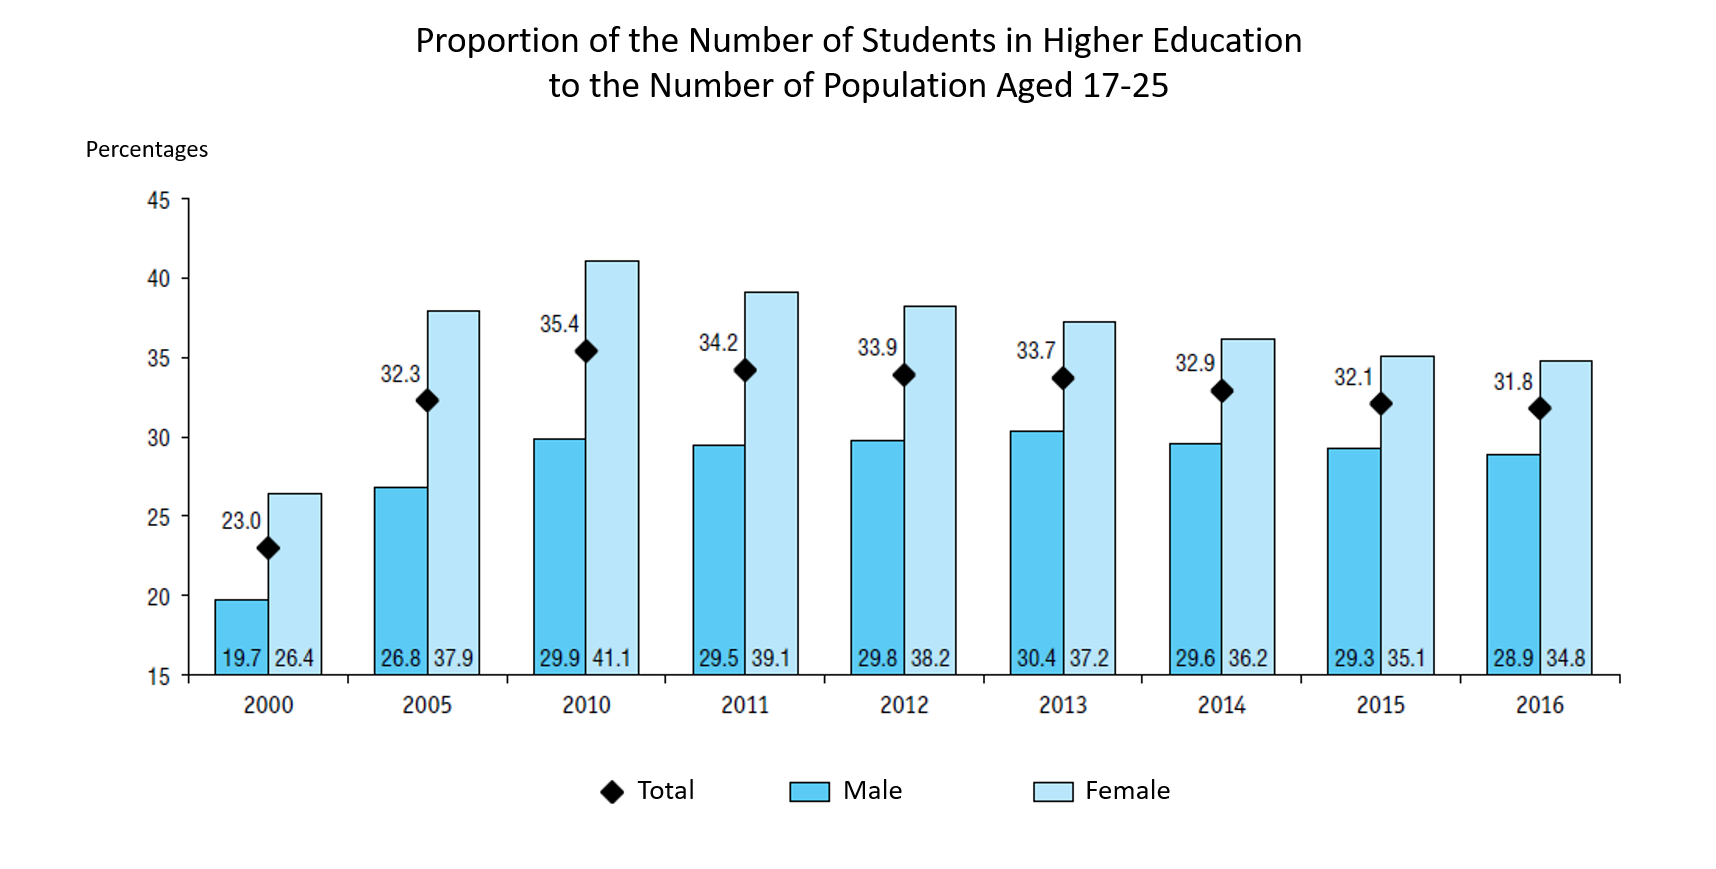
\includegraphics[width=370pt]{graph_1b.png}
\end{figure}
\begin{itemize}
	\vspace*{-0.3in}
	\item Even as university enrollment had expanded rapidly since 2000, it appears to have peaked and then declined.
\end{itemize}
\end{frame}
	
%%%%%%%%%%
\begin{frame}{Motivation}{Labor Force Distribution by Educational Level (Rosstat)}
	\begin{center}
		\centering
		\vspace*{-0.2in}
		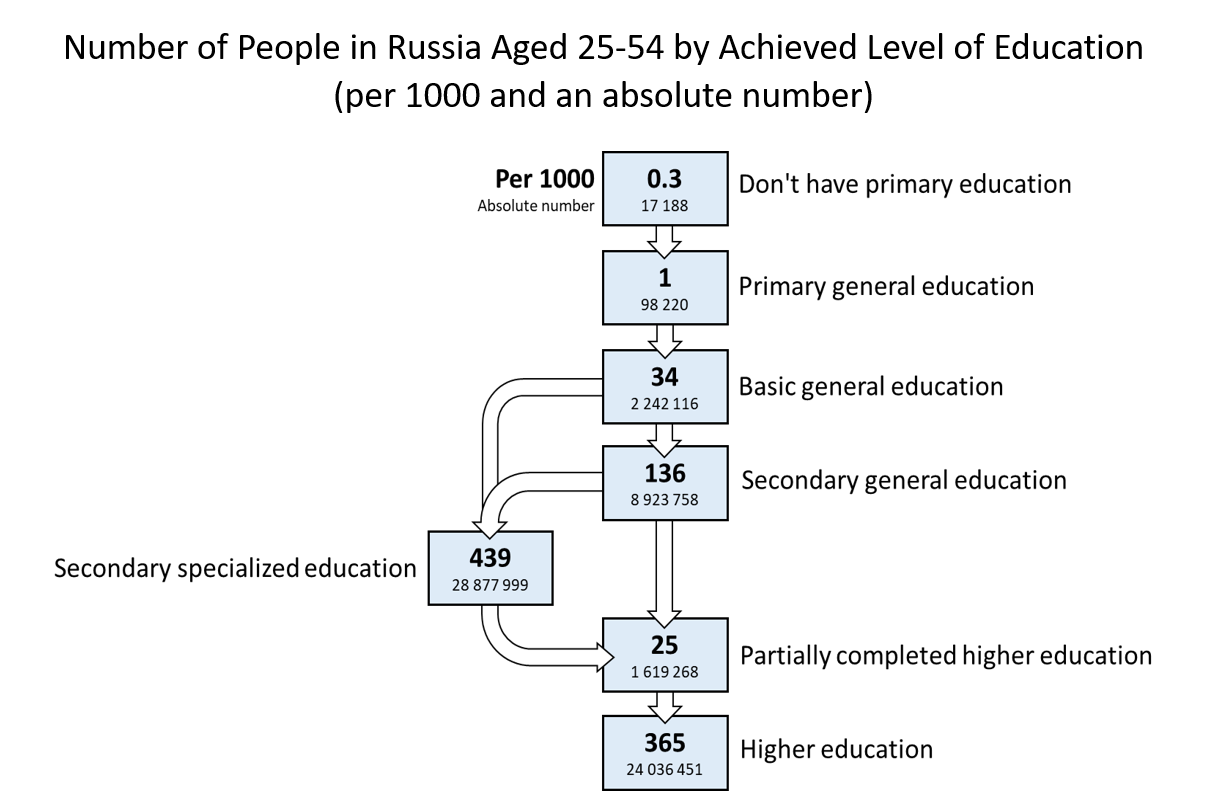
\includegraphics[width=300pt]{graph_1c.png}
	\end{center}
\end{frame}

%%%%%%%%%%
\begin{frame}{Motivation}{PISA Mean Scores for Russian Federation (OECD/PISA)}
\begin{figure}
	\centering
	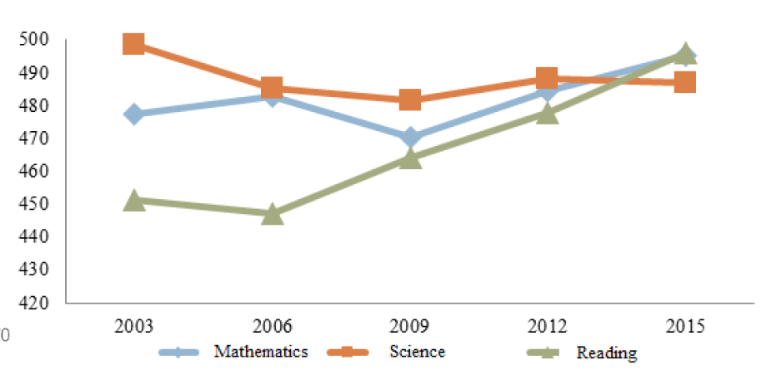
\includegraphics[width=300pt]{graph_1d.png}
\end{figure}
\begin{itemize}
	\item On cognitive attainment at Grade\,9, Russian students are already at par with OECD students.
\end{itemize}
\end{frame}

%%%%%%%%%%
\section{Returns to Education in the Russian Federation}
\subsection{Data and Methods}
\begin{frame}{Returns to Education in the Russian Federation}{Data and Methods}
	\begin{itemize}
		\item \textbf{Data:} the Russian Longitudinal Monitoring Survey (RLMS), 1994-2018.
		\item \textbf{Sample:} working individuals aged 25-64 who are out of school and have positive labor market experience and income.
		\item \textbf{Methods:} Mincerian equations estimation:
		\begin{multline}
		Log(Wage) = b_0 + b_1\cdot Education + b_2\cdot Experience + \\
		+ b_3\cdot Experience^2 + b_4\cdot Gender + \epsilon
		\end{multline}
		
		\begin{multline}\label{eq:1.2} 
		Log(Wage) = a_0 + a_1\cdot D_{Vocational} + a_2\cdot D_{Higher} + \\
		+ a_3\cdot Experience + a_4\cdot Experience^2 + a_5\cdot Gender + \epsilon
		\end{multline}
	\end{itemize}
\end{frame}

%%%%%%%%%%
\subsection{Results}
\begin{frame}{Results on Returns to Education in Russia}{Rates of Overall and Gender-wise Returns to Education in 1994-2018}
	\centering
	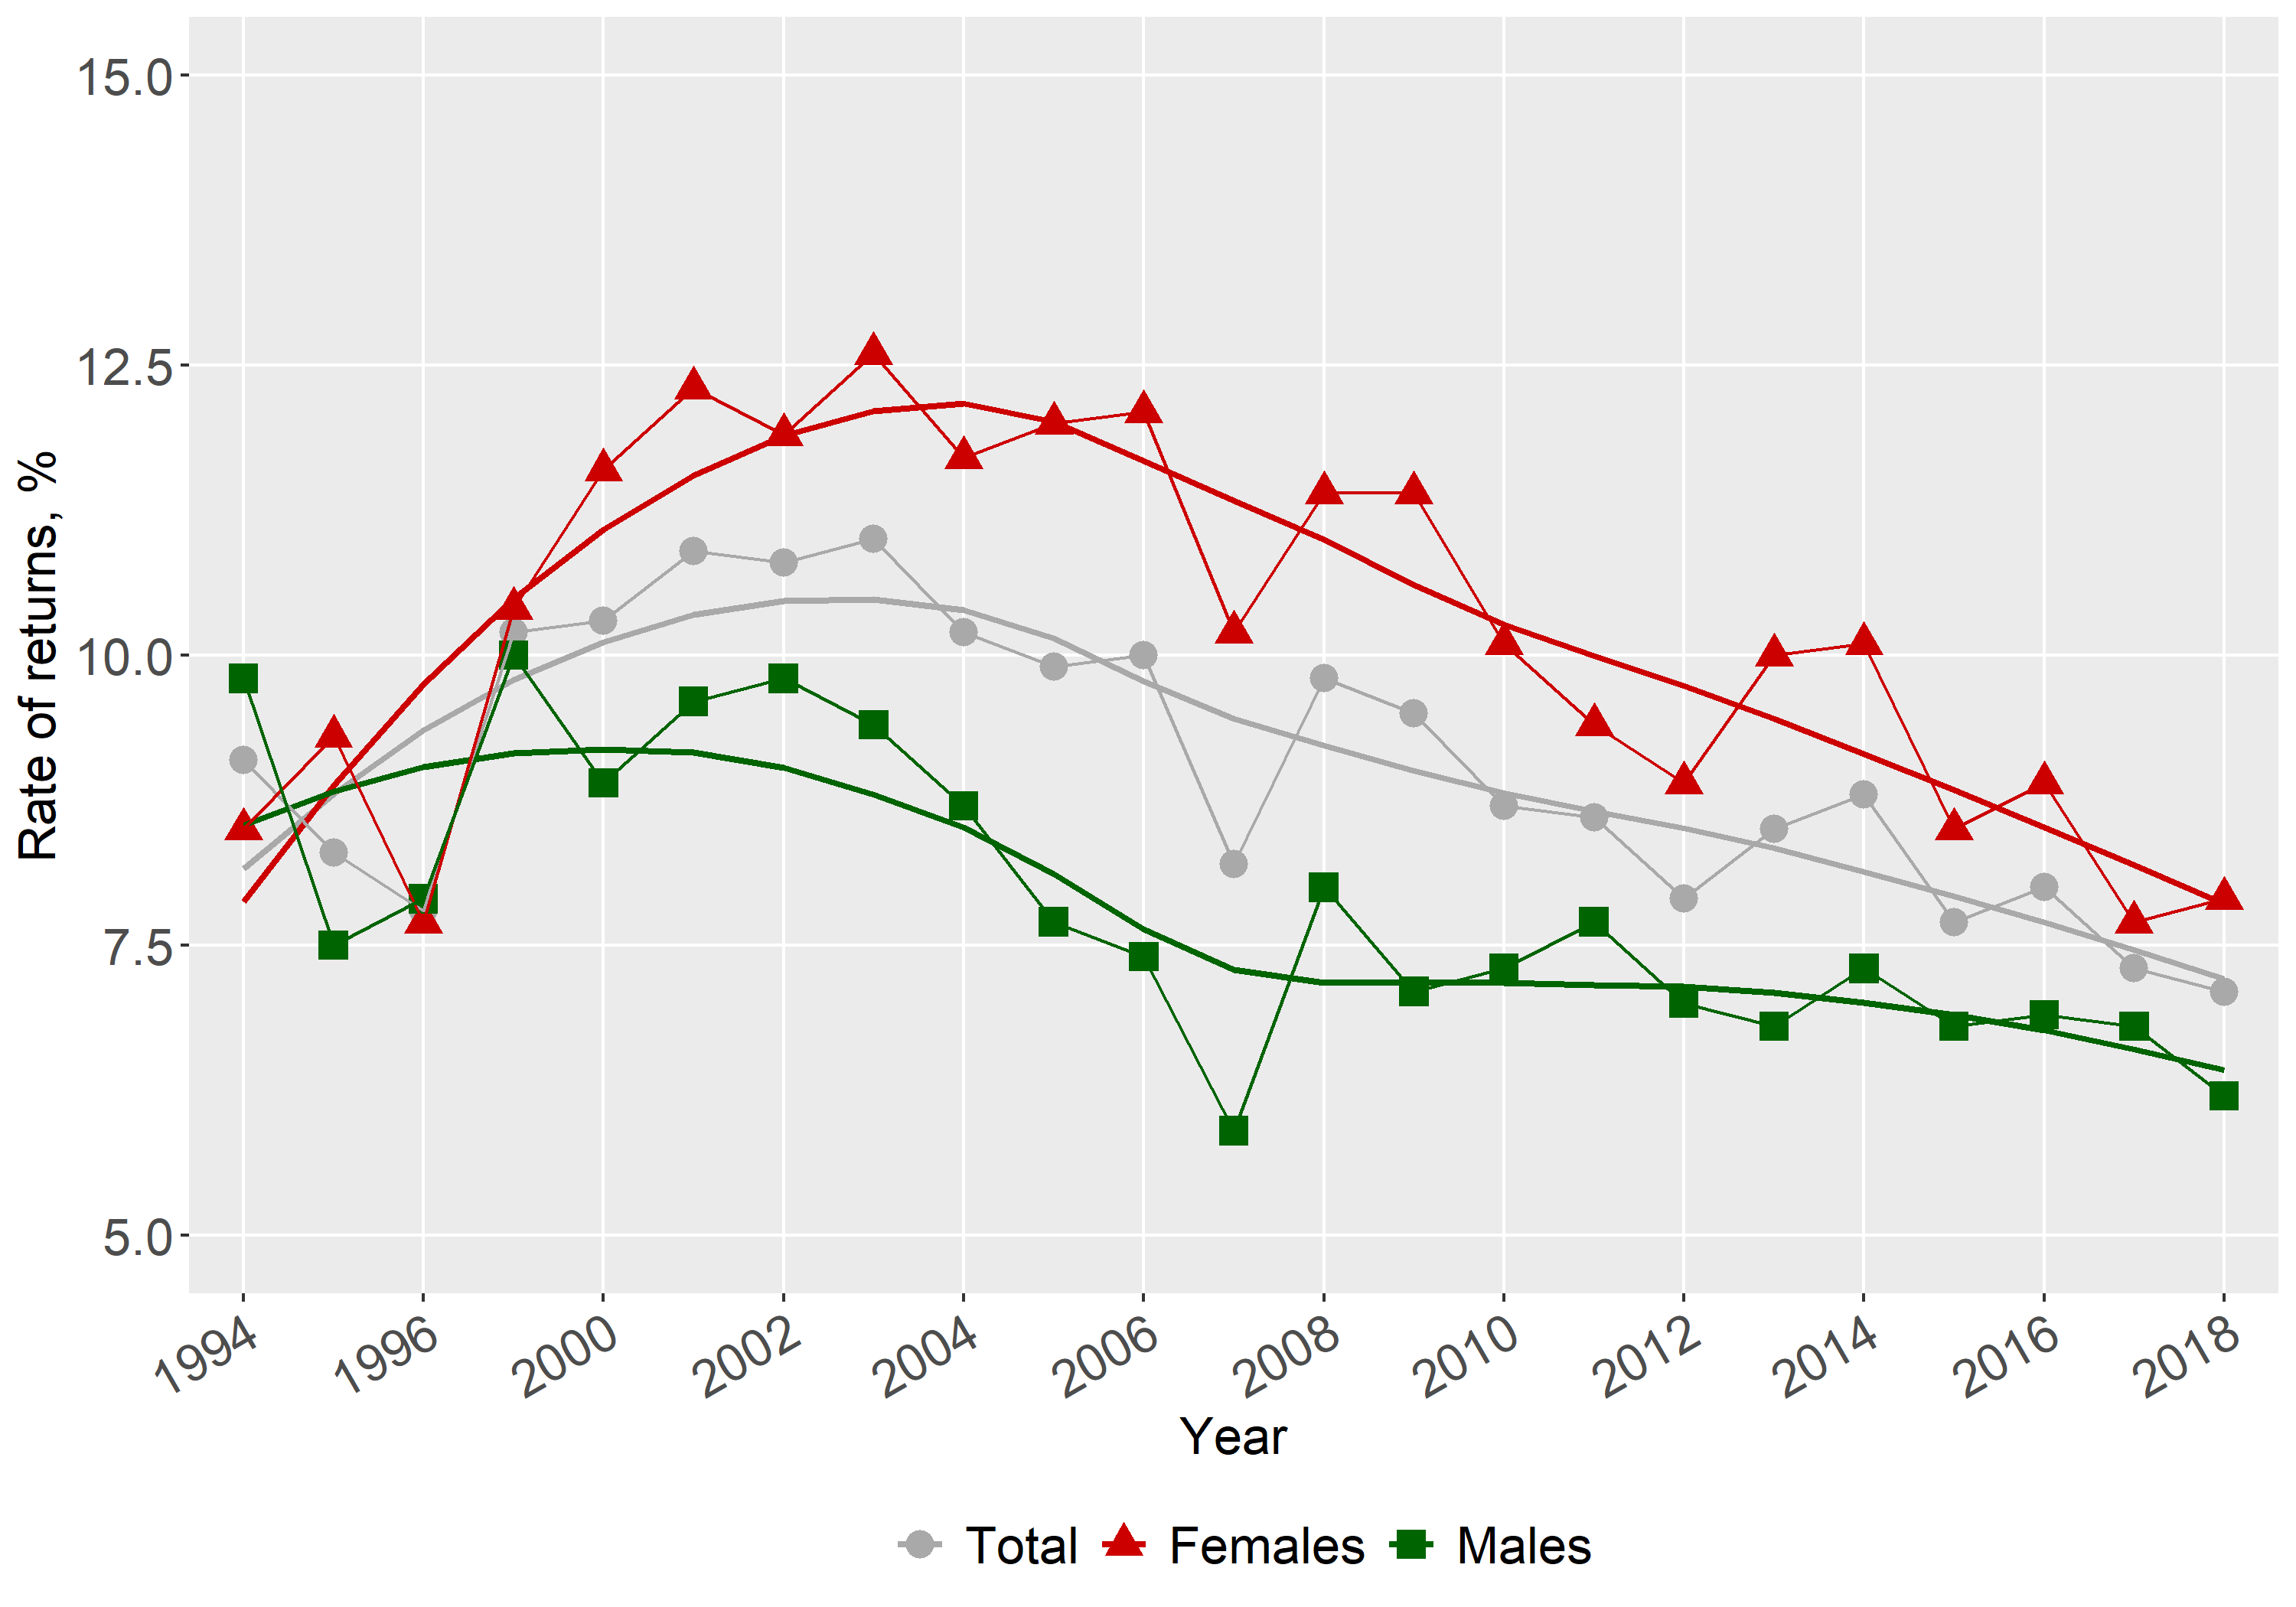
\includegraphics[width=260pt, height=200pt]{re_edu.png}
\end{frame}

%%%%%%%%%%
\begin{frame}{Results on Returns to Education in Russia}{Co-movement of Vocational and Higher Education and Enrollment in Higher Education}
\begin{figure}
	\centering
	\subfloat[Rate of Returns to Education]{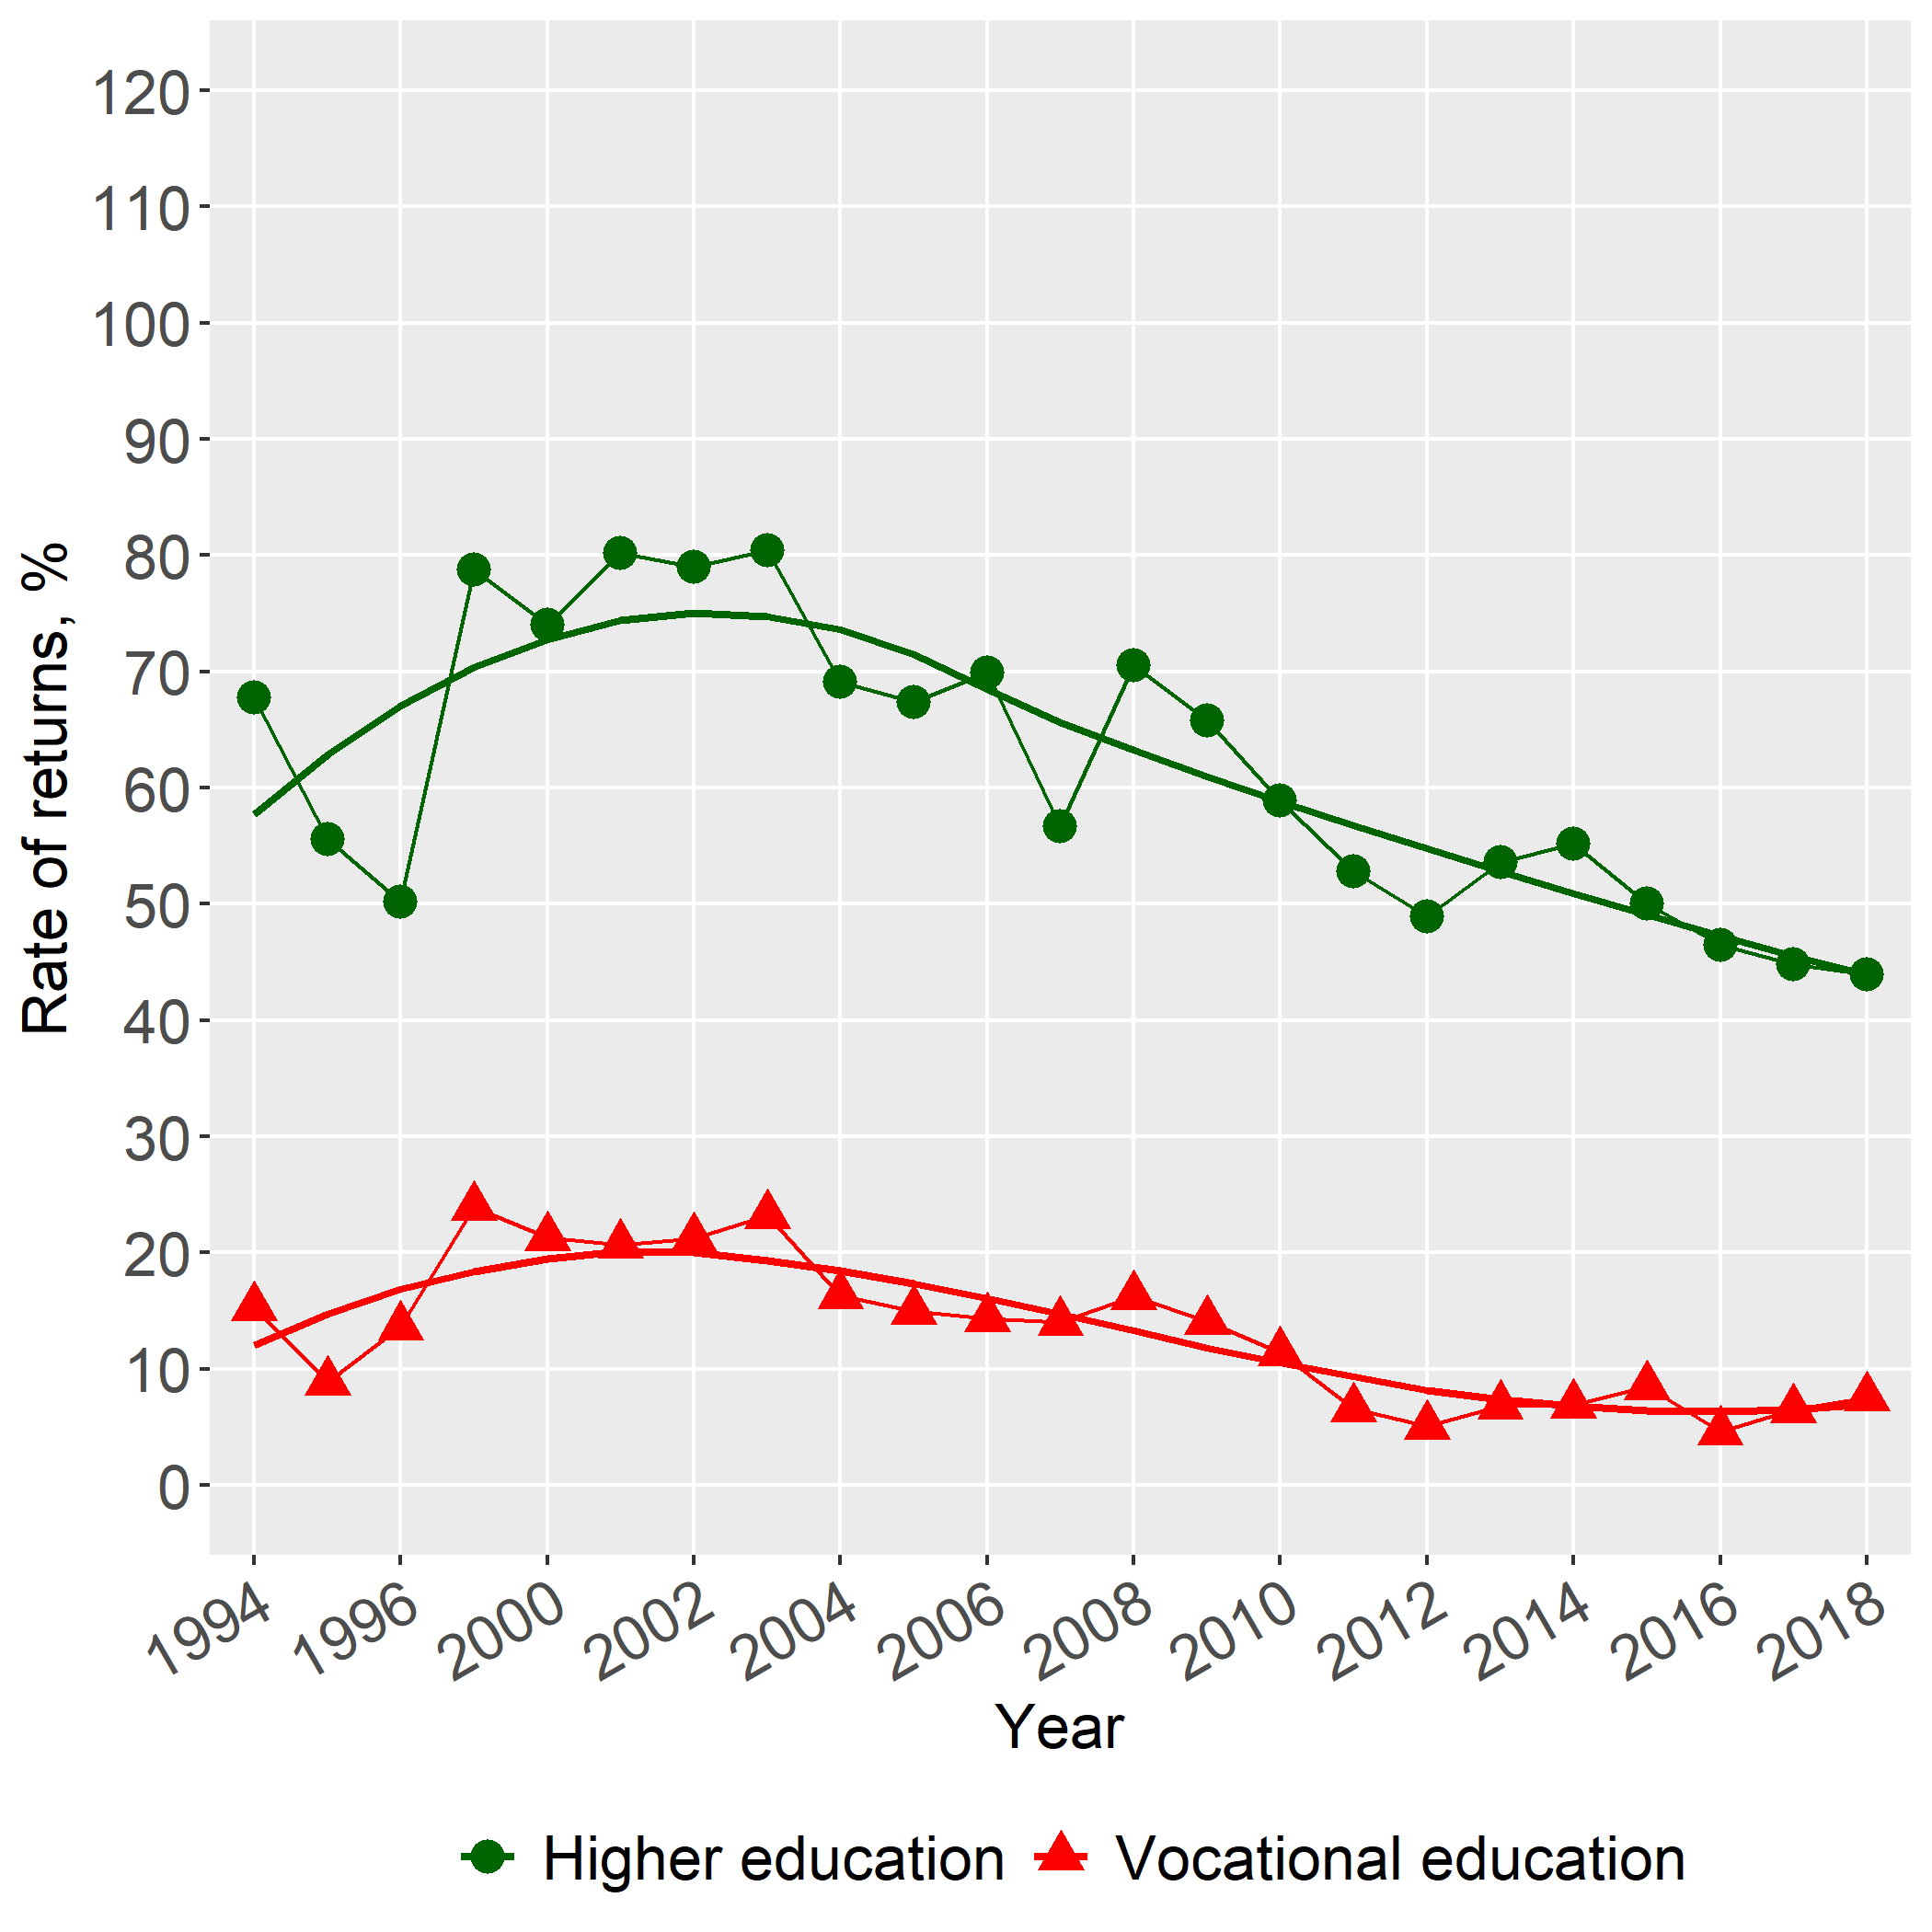
\includegraphics[width=150pt]{re_HE_all.png}}
	\hfill
	\subfloat[Enrollment in Higher Education]{\vspace*{0.5in} 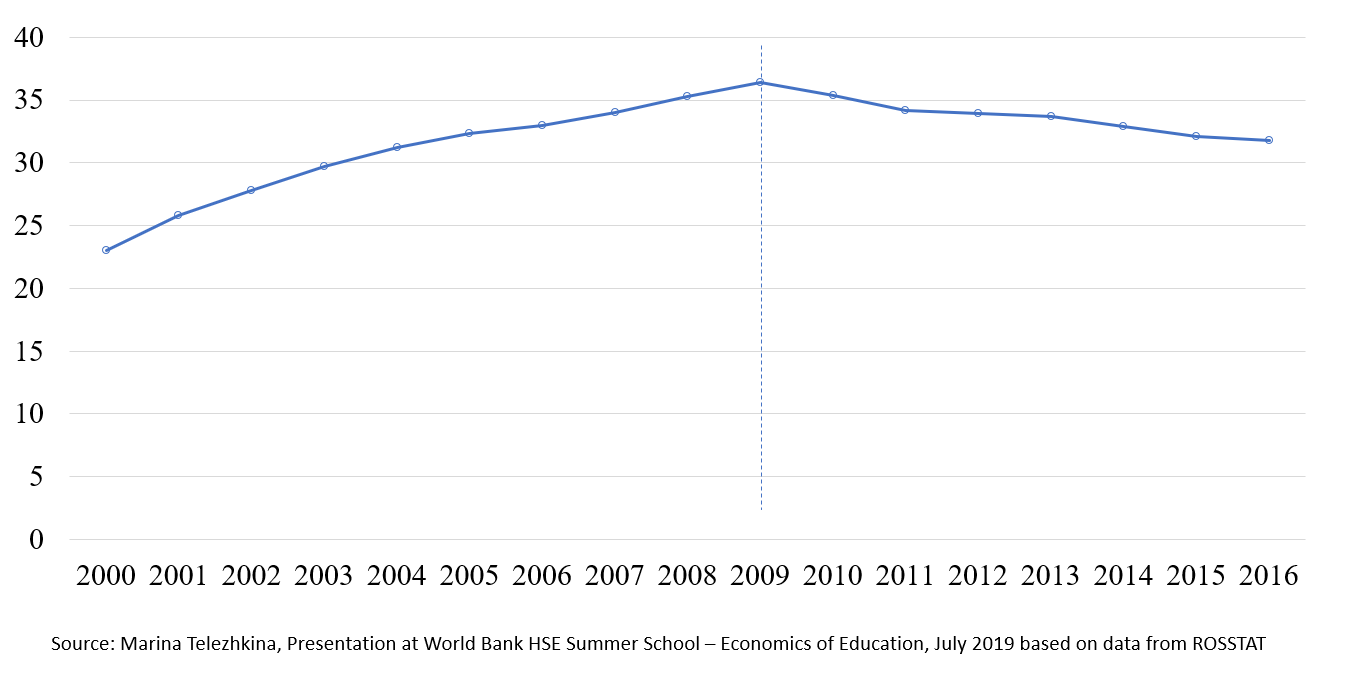
\includegraphics[width=180pt]{telezhkina.png}}
\end{figure}
\begin{itemize}
	\vspace*{-0.2in}
	\item The graphs display downturn in returns reflected in enrollments, with the peak in enrollments coming about 10 years later.
\end{itemize}
\end{frame}

%%%%%%%%%%
\begin{frame}{Results on Returns to Education in Russia}{Co-movement of Vocational Education and Higher Education by Gender}
\begin{figure}
		\centering
		\subfloat[Females]{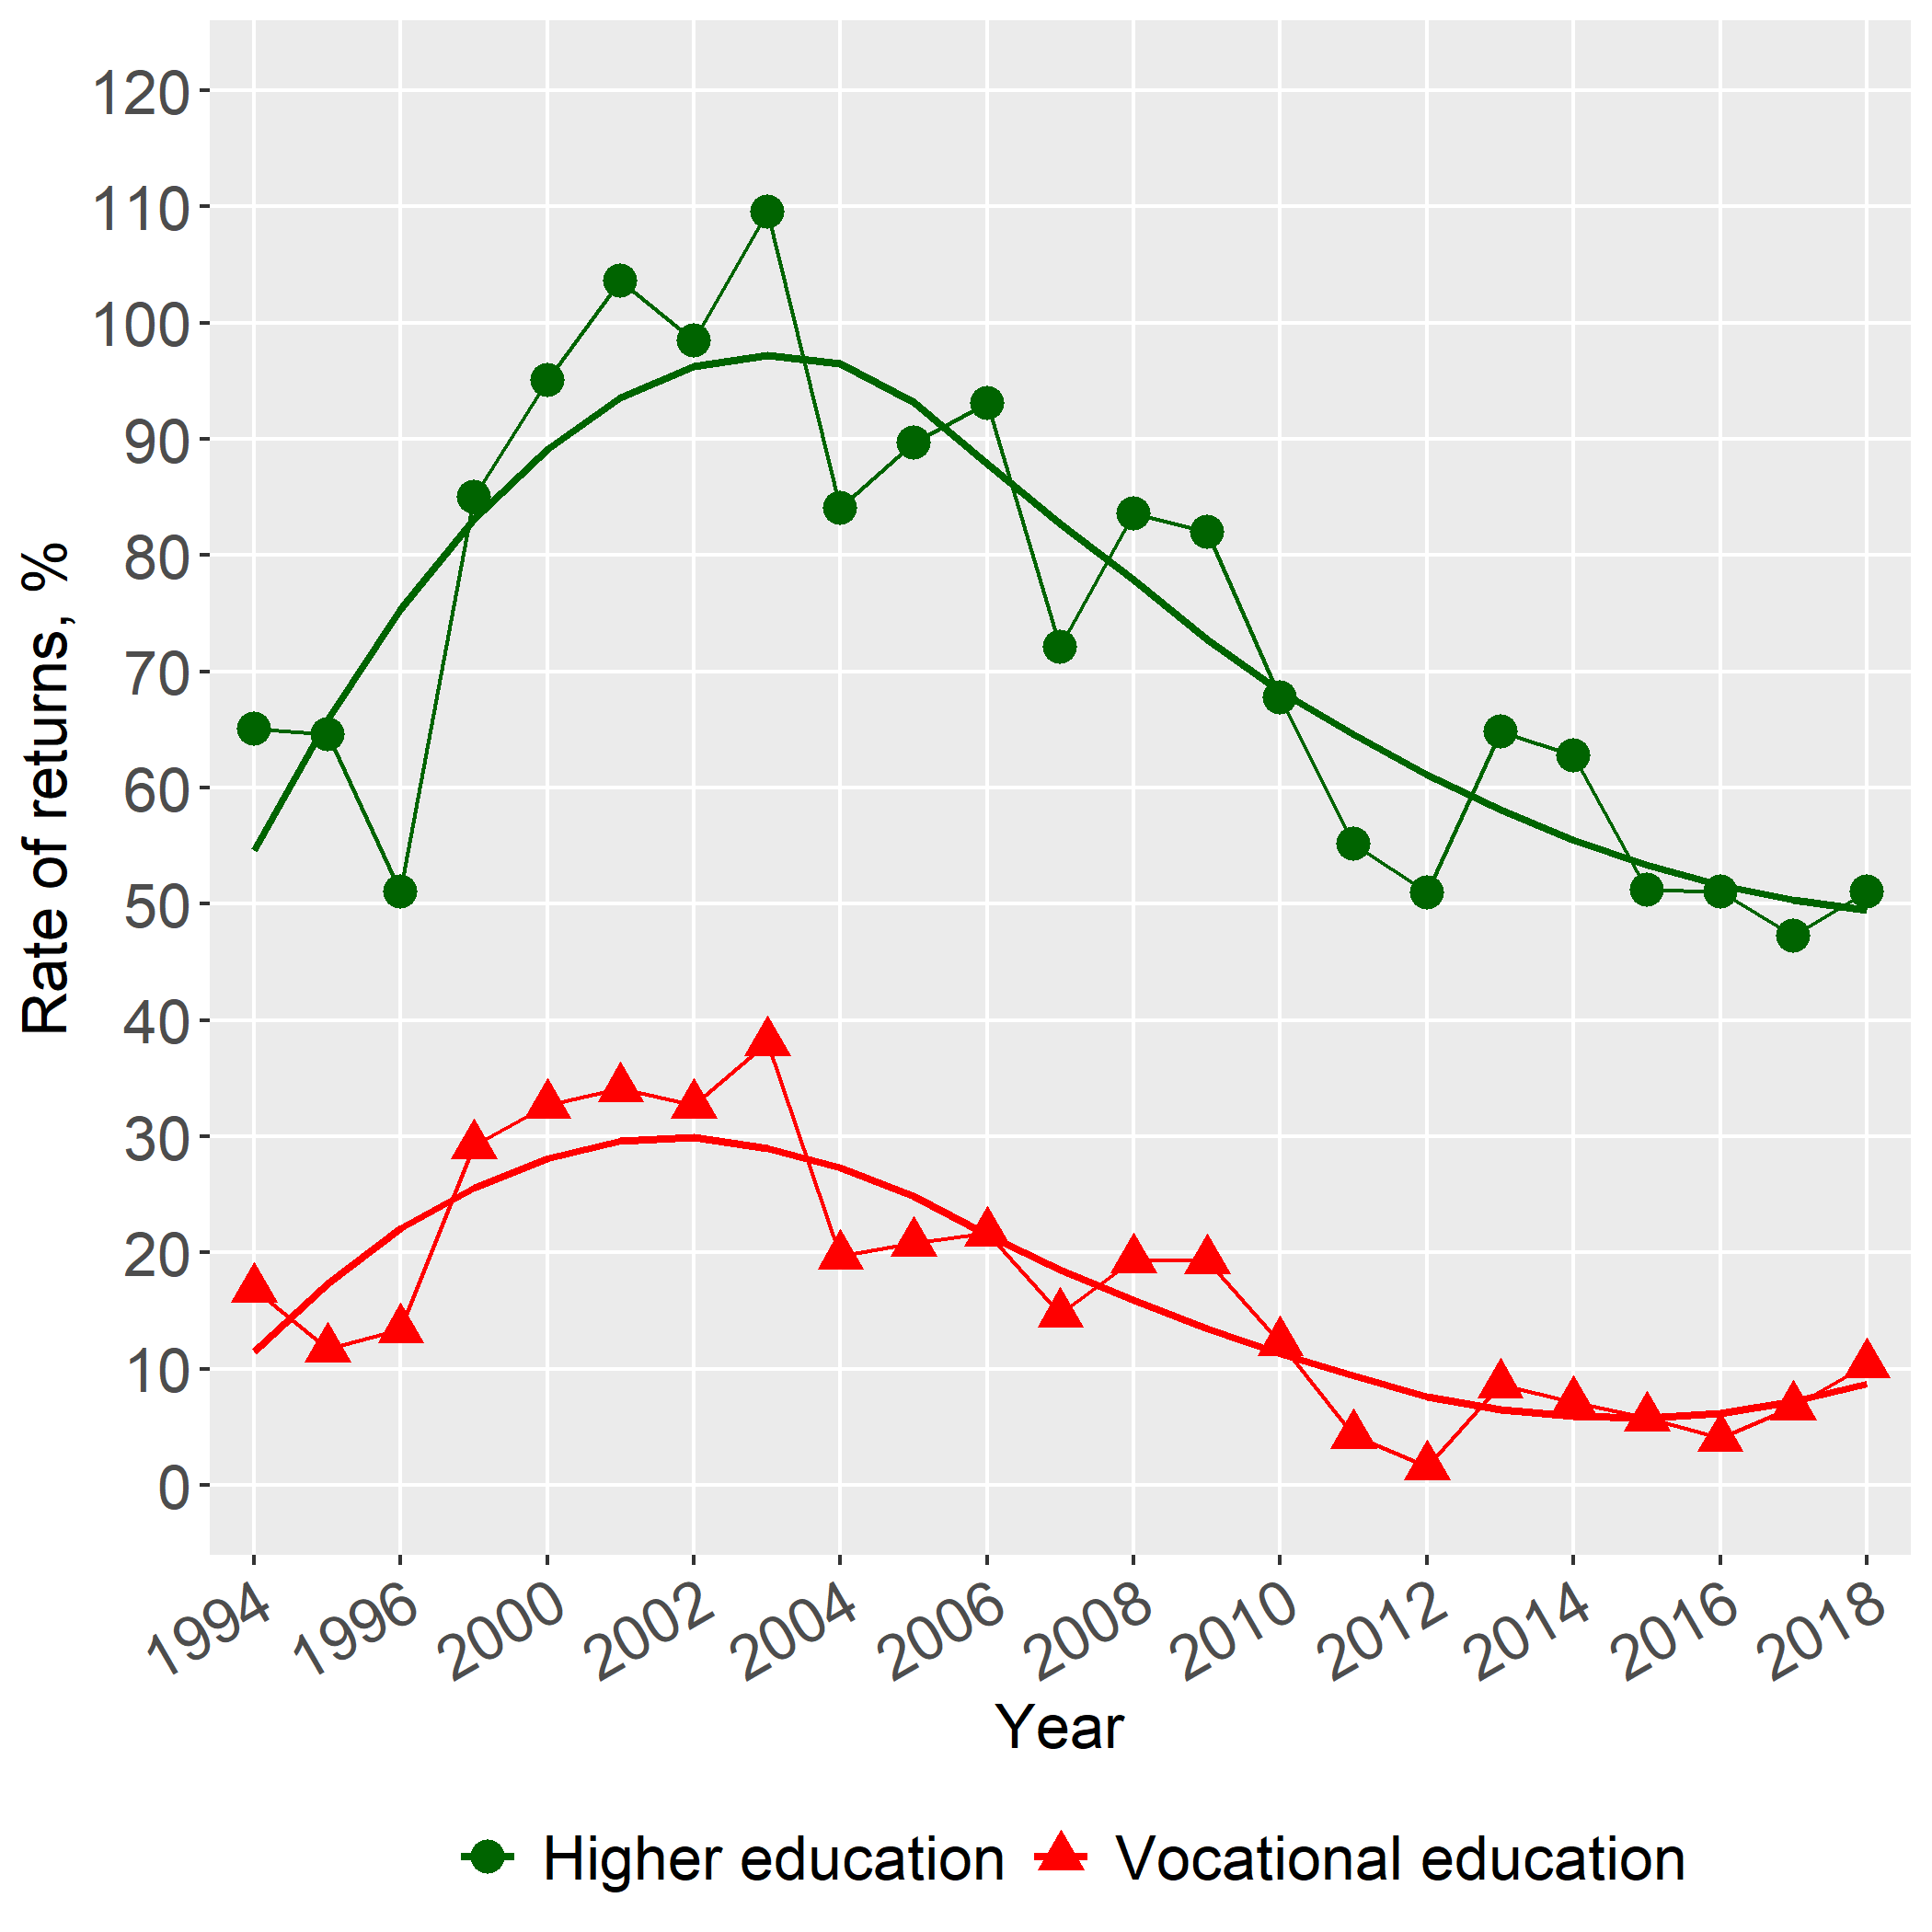
\includegraphics[width=150pt]{re_HE_f.png}}
		\hfill
		\subfloat[Males]{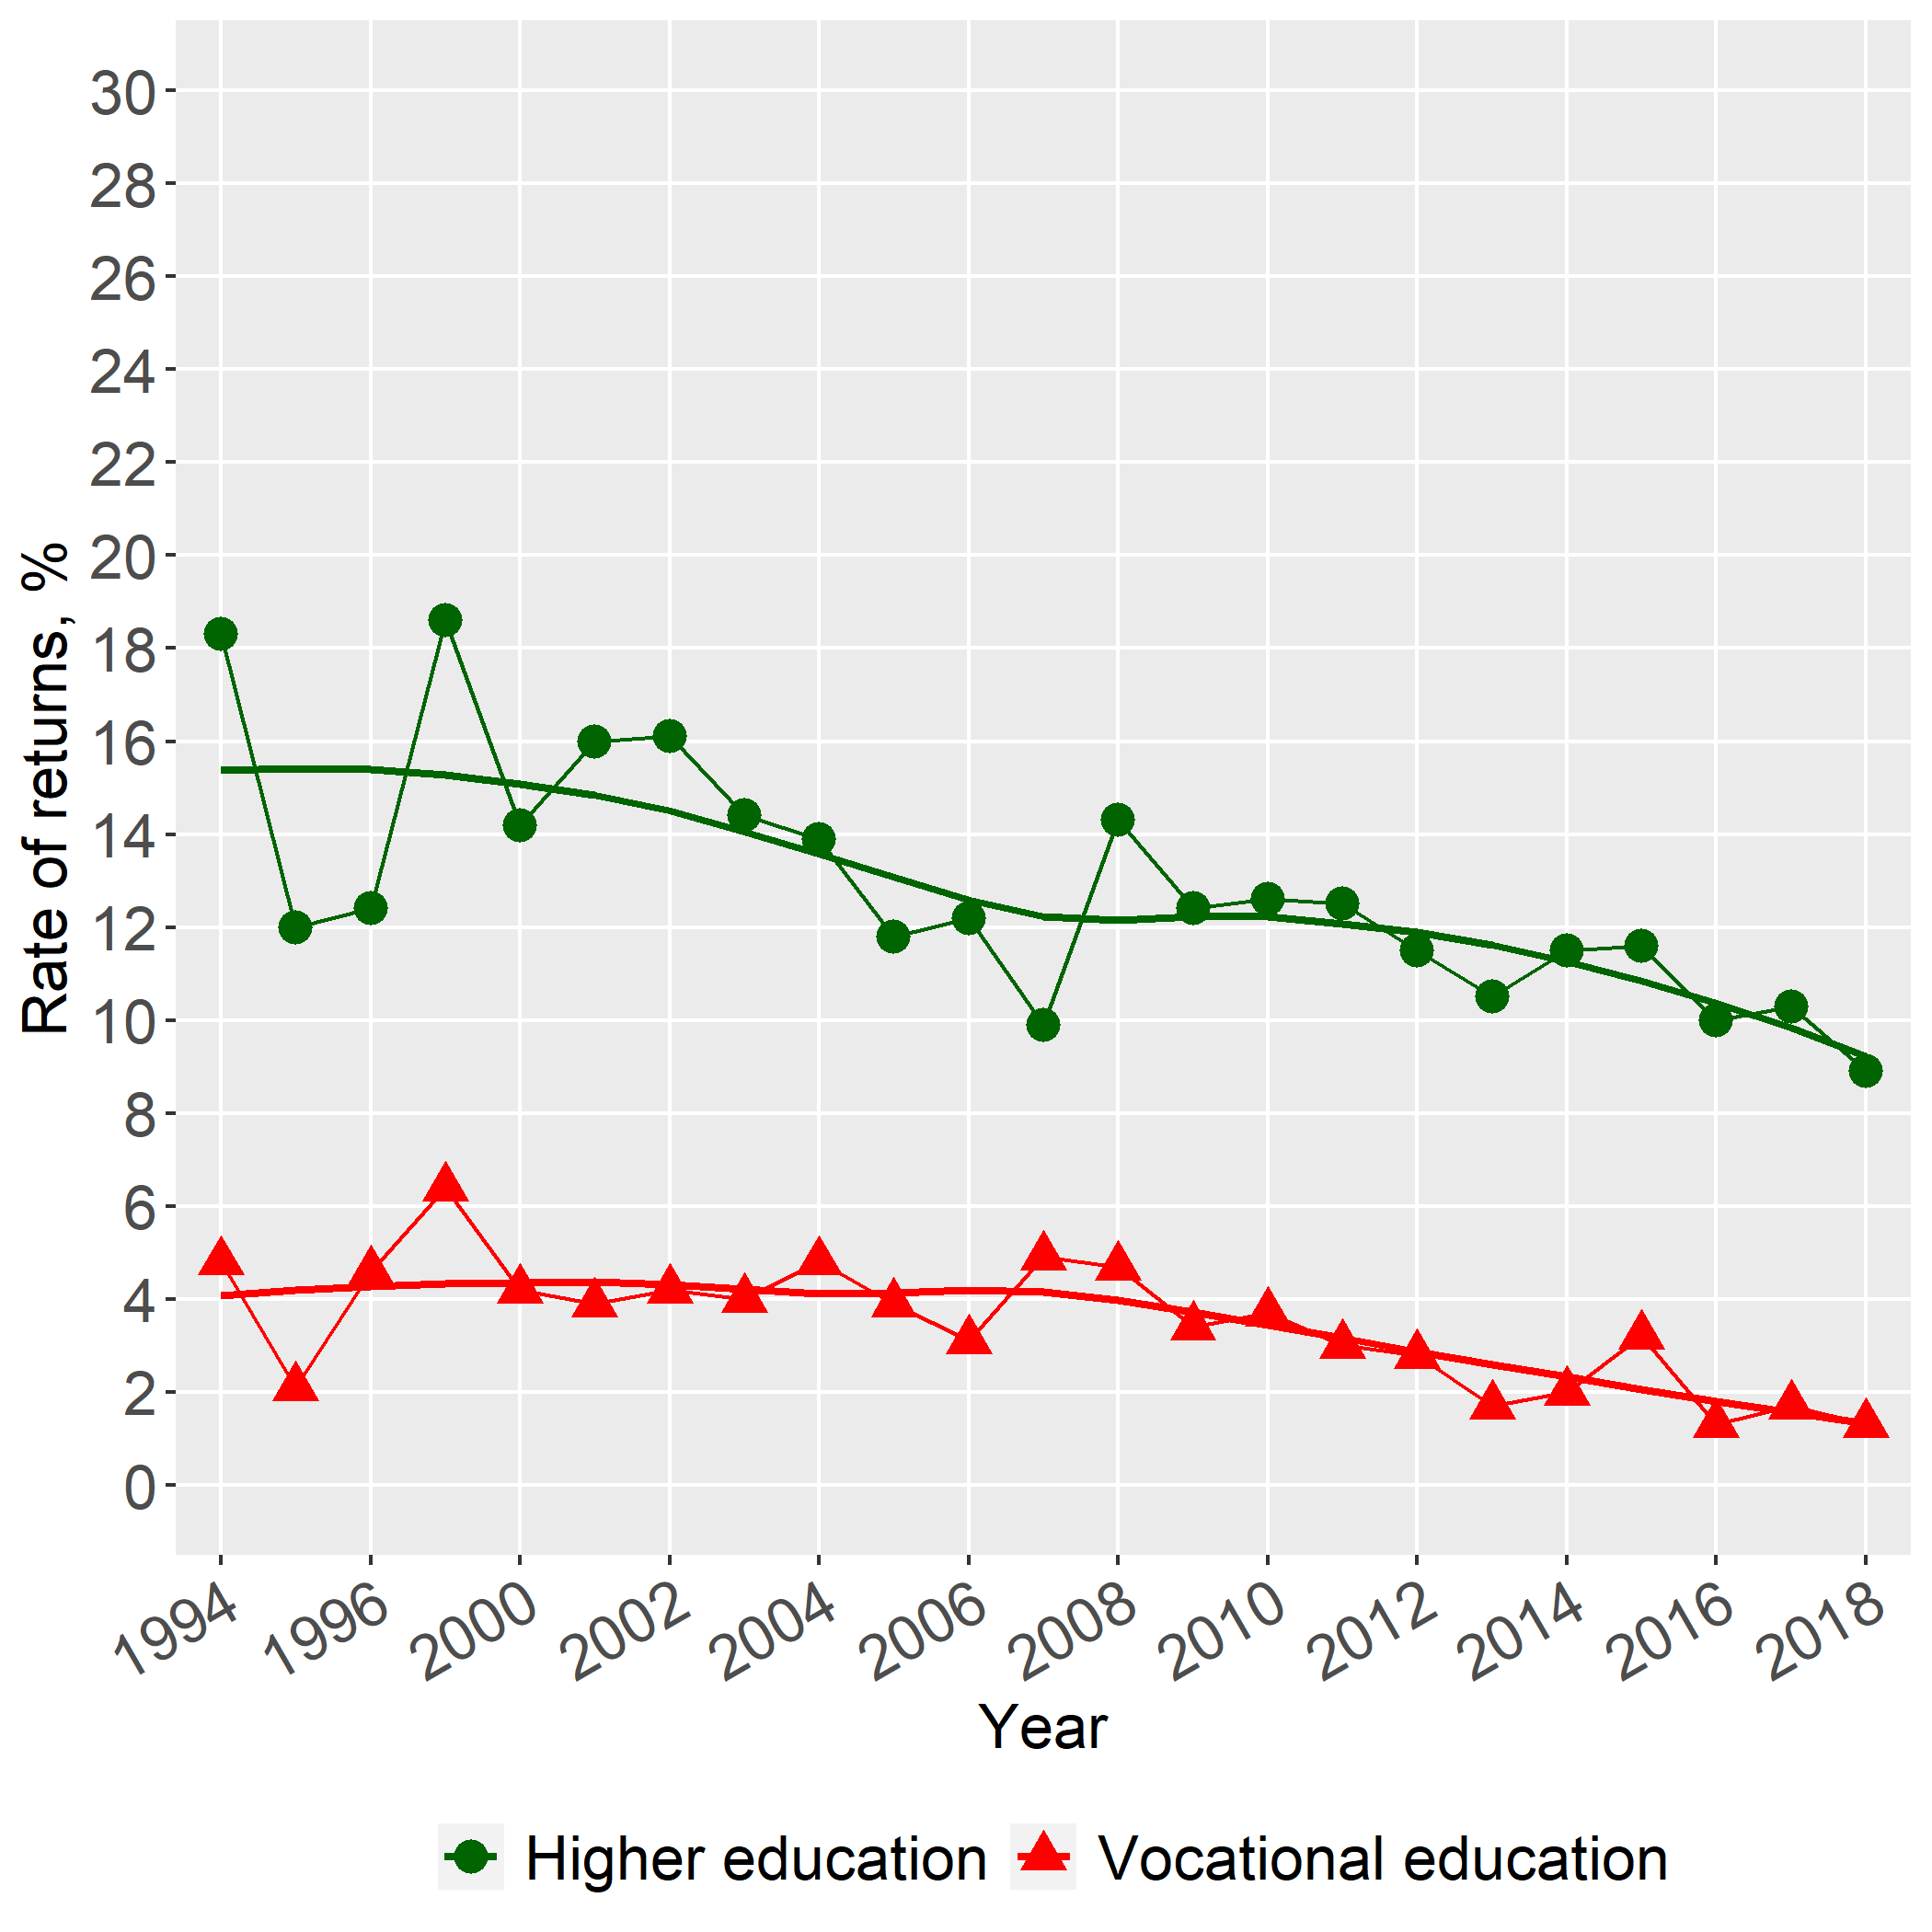
\includegraphics[width=150pt]{re_HE_m.png}}
	\end{figure}
\begin{itemize}
	\vspace*{-0.2in}
	\item Returns for males are almost flat.
	\item Returns for females show a \textit{concave} pattern.
\end{itemize}
\end{frame}

%%%%%%%%%%
\section{Depreciation of Human Capital in Russia}
\subsection{Analytical Treatment of Depreciation}
\begin{frame}{Depreciation of Human Capital in Russia}{Analytical Treatment of Depreciation}
	Two kinds of depreciation or \textit{loss of productive potential of human capital} \citep{neuman_091._1995}:
	\begin{itemize}
	\item \textbf{External depreciation} (``obsolescence" or ``vintage effect"): due to an overall upgrading of technology or the operation of other market forces that lowers the value of education or training obtained in a previous period.
	\item \textbf{Internal depreciation:} due to deterioration of physical and mental abilities of an individual due to the progression of a person's age.
	\end{itemize}
\end{frame}

%%%%%%%%%%
\begin{frame}{Depreciation of Human Capital in Russia}{Neuman-Weiss Vintage Effects by Education Levels}
\begin{figure}
	\centering
	\subfloat[Higher Education]{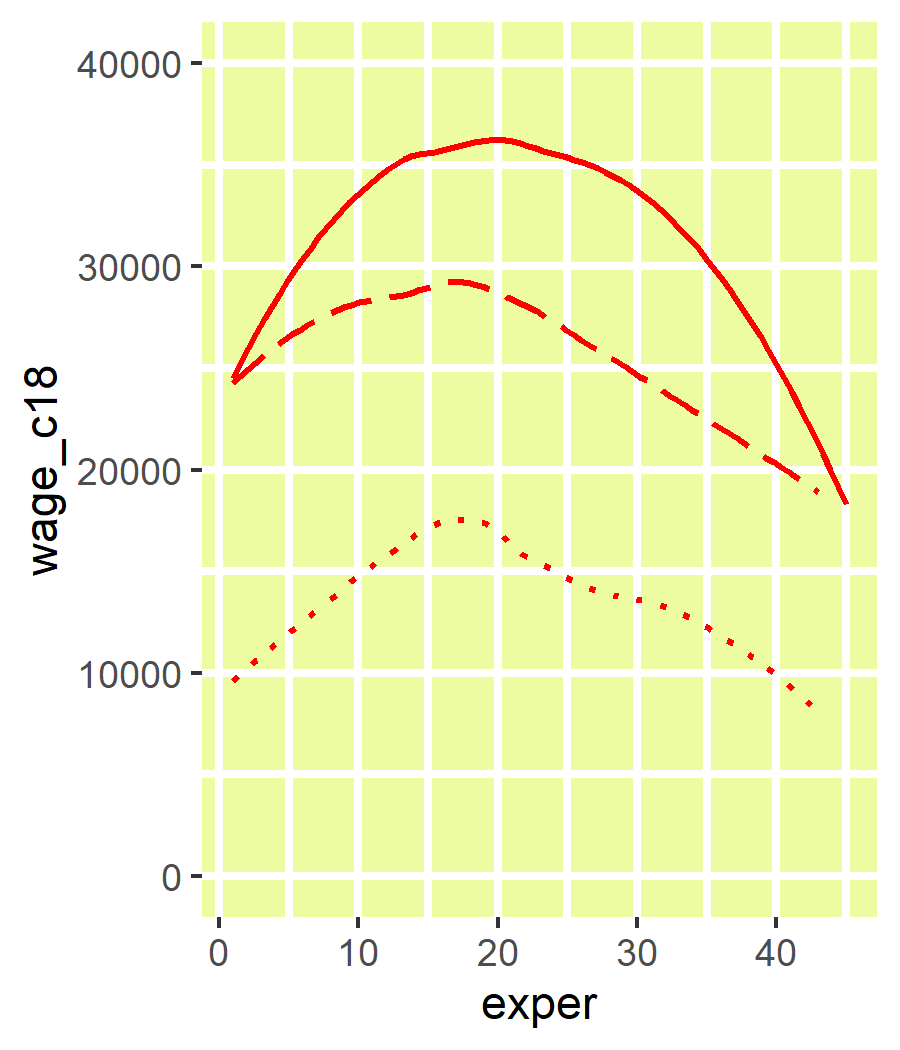
\includegraphics[width=110pt]{dp01_he.png}}
	\hfill
	\subfloat[Vocational Education]{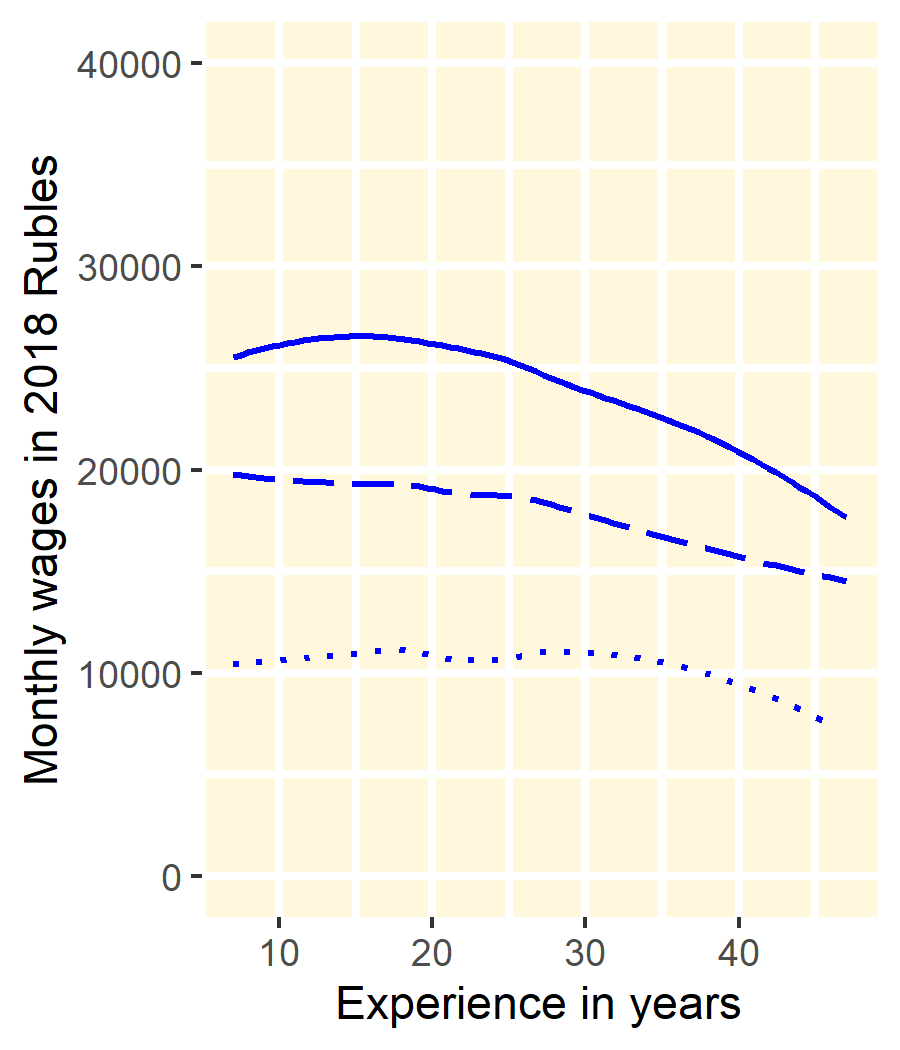
\includegraphics[width=110pt]{dp01_ve.png}}
	\hfill
	\subfloat[Secondary Education]{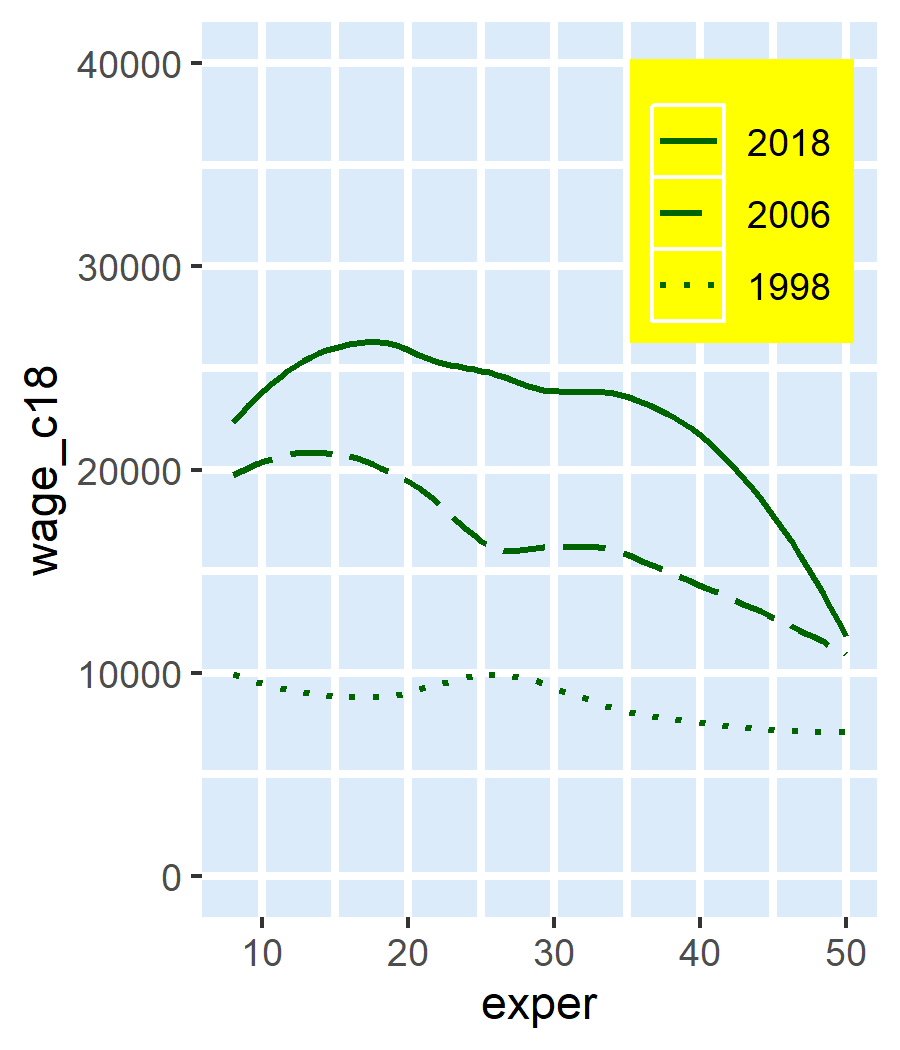
\includegraphics[width=110pt]{dp01_se.png}}
\end{figure}
\begin{itemize}
	\item A clear concave downwards profile is only for Higher Education.
	\item The concave tendency is less pronounced for the other two levels of Vocational and Secondary education.
\end{itemize}
\end{frame}

%%%%%%%%%%
\begin{frame}{Depreciation of Human Capital in Russia}{Neuman-Weiss Vintage Effects by Year}
	\begin{figure}
		\centering
		\subfloat[1998]{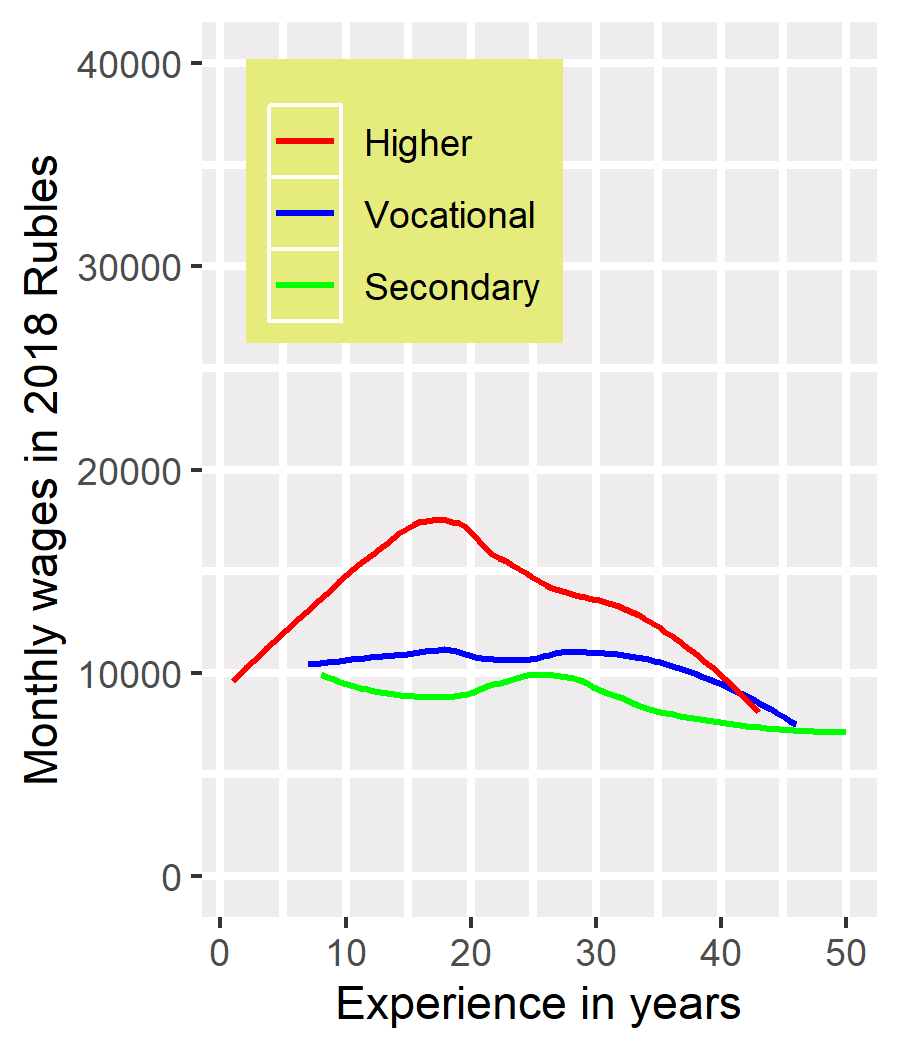
\includegraphics[width=110pt]{dp01_98.png}}
		\hfill
		\subfloat[2006]{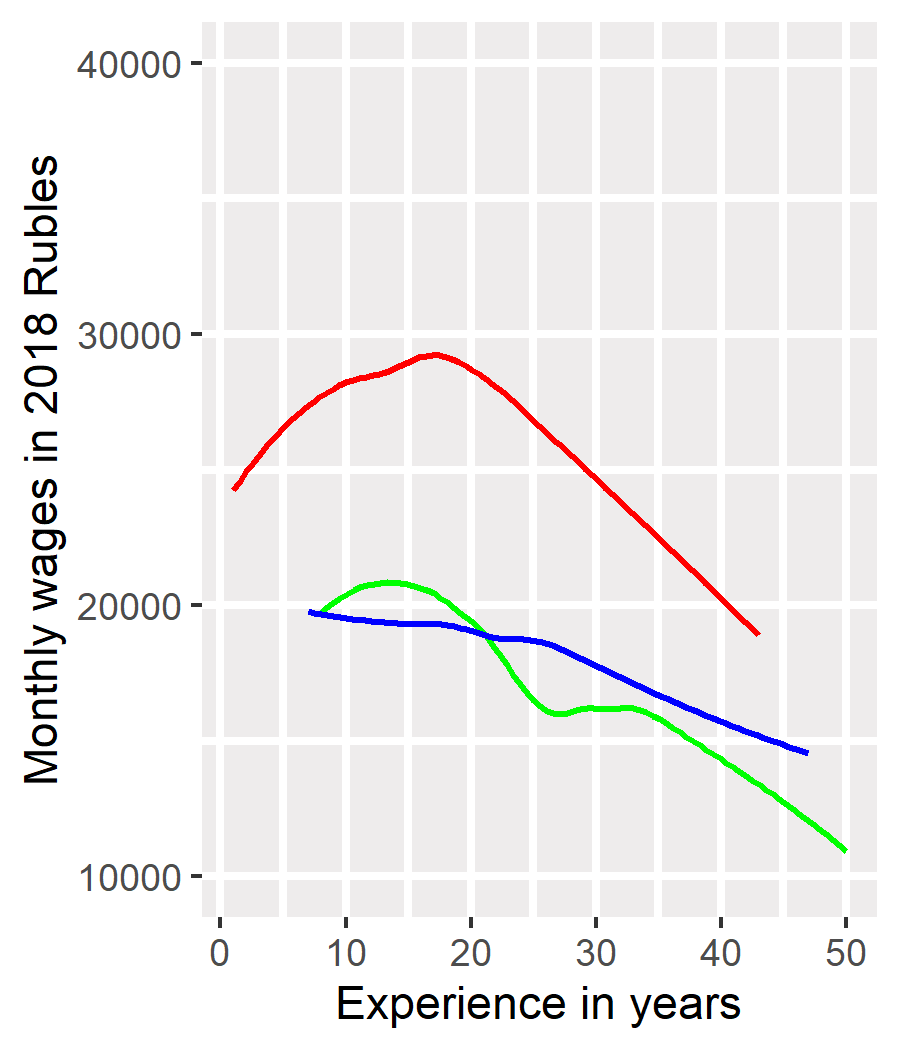
\includegraphics[width=110pt]{dp01_06.png}}
		\hfill
		\subfloat[2018]{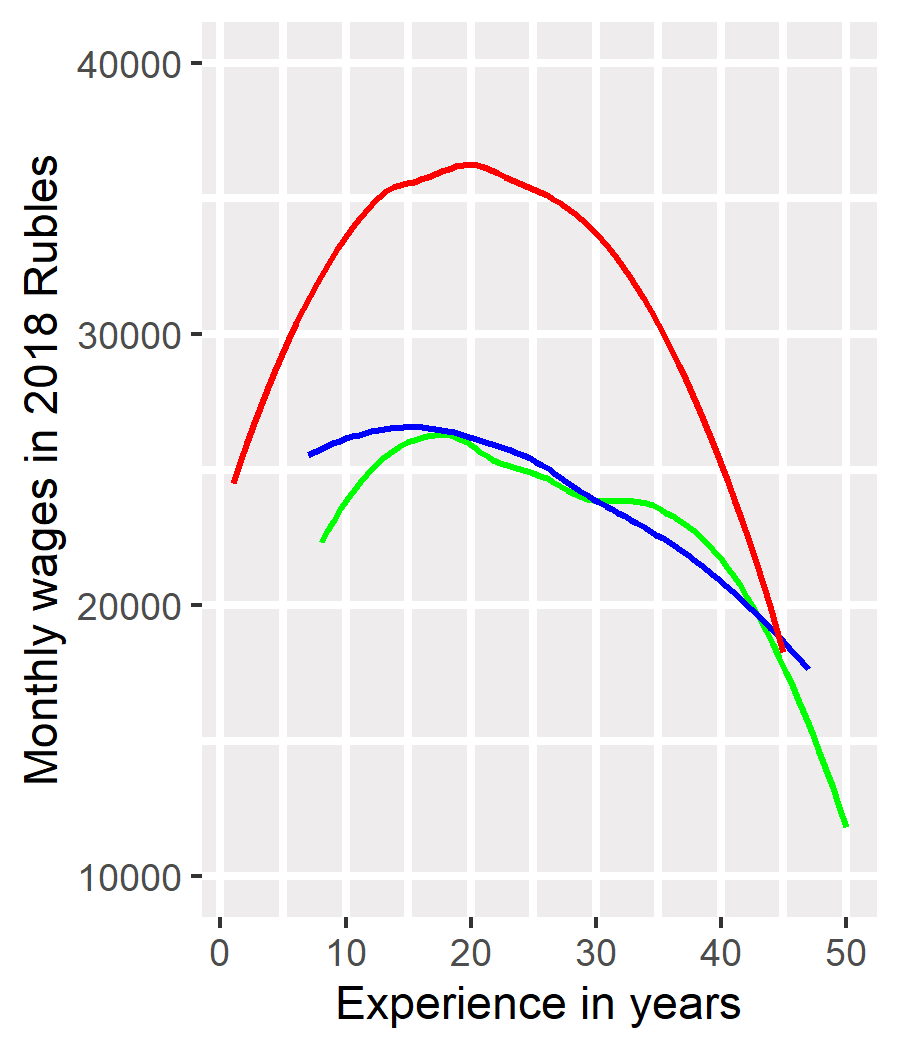
\includegraphics[width=110pt]{dp01_18.png}}
	\end{figure}
	\begin{itemize}
		\item The premium for university education over the other two levels does narrow at higher levels of experience.
	\end{itemize}
\end{frame}

%%%%%%%%%%
\begin{frame}{Depreciation of Human Capital in Russia}{Murillo Methods}
\begin{itemize}
	\item \citet{murillo_172._2006} implemented a variation of the \citet{neuman_091._1995} model with a focus on
	empirical implementation to Spain.
	\item In a nutshell, the model can be expressed as follows:
	
	\begin{equation}
	log(W) = \alpha +  \beta_{1}S + \pi_{1}TS + \beta_{2}T + \pi_{2}T^{2} 
	\end{equation}
	where $T$ is years of experience, $S$ is years of schooling, $\alpha$, $\beta_{1}$, $\beta_{1}$, $\pi_{1}$, $\pi_{2}$ are regression coefficients.
	\vspace{2pt}
	\item The depreciation rate during $T$ years applied to schooling can be computed as $\pi_{1}S $ and the depreciation rate applied to experience as $ 2\pi_{2}T$.
\end{itemize}
\end{frame}

%%%%%%%%%%
\subsection{Estimation Results}
\begin{frame}{Depreciation of Human Capital in Russia}{Average Depreciation Rate (DR) by Years}
	\fontsize{6}{8}\selectfont
	\begin{tabularx}{\textwidth}{rlrrrrrrc}
		\hline
		\multicolumn{9}{l}{\textbf{Panel A: Whole Sample}} \\
		\hline
		& \textbf{Statistic} & \textbf{1994} & \textbf{1998} & \textbf{2003} & \textbf{2006} & \textbf{2012} & \textbf{2018} &  \\ 
		\hline
		1 & Experience, mean   & 21.41 & 22.32 & 22.20 & 22.24 & 22.52 & 22.52 & \\
		2 & Education, mean & 12.70 & 12.69 & 12.79 & 12.79 & 12.95 & 13.27 &\\
		\hline
		3 & DR Experience, \% & 1.87 & 1.55 & 1.04 & 0.50 & 1.37 & 1.63 & 
		\graph{1}{1}{C:/Country/Russia/Data/SEASHELL/SEABYTE/Edreru/wp1/sparklines/all2-1} \\ 
		4 & DR Education, \% & 2.80 & 2.71 & 0.11 & 0.00 & 0.00 & 0.00 &
		\graph{1}{1}{C:/Country/Russia/Data/SEASHELL/SEABYTE/Edreru/wp1/sparklines/all2-2} \\ 
		5 & DR Human Capital, \% & 4.67 & 4.26 & 1.15 & 0.50 & 1.37 & 1.63 & 
		\graph{1}{1}{C:/Country/Russia/Data/SEASHELL/SEABYTE/Edreru/wp1/sparklines/all2-3}\\ 
		\hline
	\end{tabularx}
	\begin{tabularx}{\textwidth}{rlrrrrrrc}
		\hline
		\multicolumn{9}{l}{\textbf{Panel B: Female Sample}} \\
		\hline
		1 & Experience, mean & 21.36 & 22.09 & 22.34 & 22.33 & 22.69 & 22.67 & \\  
		2 & Education, mean & 12.76 & 12.85 & 12.98 & 13.05 & 13.24 & 13.58 & \\ 
		\hline
		3 & DR Experience, \% & 2.46 & 2.57 & 1.62 & 0.78 & 1.23 & 1.52 & 
		\graph{1}{1}{C:/Country/Russia/Data/SEASHELL/SEABYTE/Edreru/wp1/sparklines/female2-1} \\  
		4 & DR Education, \% & 3.81 & 5.31 & 3.97 & 0.00 & 0.00 & 0.00 & 
		\graph{1}{1}{C:/Country/Russia/Data/SEASHELL/SEABYTE/Edreru/wp1/sparklines/female2-2} \\
		5 & DR Human Capital, \% & 6.27 & 7.88 & 5.59 & 0.78 & 1.23 & 1.52 & 
		\graph{1}{1}{C:/Country/Russia/Data/SEASHELL/SEABYTE/Edreru/wp1/sparklines/female2-3} \\ 
		\hline
	\end{tabularx}
	\begin{tabularx}{\textwidth}{rlrrrrrrc}
		\hline
		\multicolumn{9}{l}{\textbf{Panel C: Male Sample}} \\
		\hline
		1 & Experience, mean & 21.47 & 22.58 & 22.02 & 22.14 & 22.31 & 22.34 & \\ 
		2 & Education, mean & 12.62 & 12.50 & 12.57 & 12.47 & 12.61 & 12.91 & \\  
		\hline
		3 & DR Experience, \% & 1.83 & 1.08 & 0.80 & 0.67 & 2.23 & 1.91 & 
		\graph{1}{1}{C:/Country/Russia/Data/SEASHELL/SEABYTE/Edreru/wp1/sparklines/male2-1} 
		\\ 
		4 & DR Education, \% & 3.96 & 2.74 & 0.91 & 0.00 & 0.00 & 0.00 & 
		\graph{1}{1}{C:/Country/Russia/Data/SEASHELL/SEABYTE/Edreru/wp1/sparklines/male2-2} 
		\\ 
		5 & DR Human Capital, \% & 5.78 & 3.82 & 1.71 & 0.67 & 2.23 & 1.91 &
		\graph{1}{1}{C:/Country/Russia/Data/SEASHELL/SEABYTE/Edreru/wp1/sparklines/male2-3} 
		\\ 
		\hline
	\end{tabularx}
\end{frame}

%%%%%%%%%%
\subsection{Arrazola's Non-Linear Least Squares Approach}

\begin{frame}{Depreciation of Human Capital in Russia}{Arrazola's Non-Linear Least Squares Approach}
\begin{itemize}
	\item \citet{arrazola_132b._2005} developed an alternative approach on the issue of human capital depreciation.
	\item The analytical solution culminates in the following equation to be estimated with Non-Linear Least Squares (the notations are taken from \citet{weber_173._2008} and \citet{weber_156._2011}):
	\begin{multline}\label{eq:2.16} 
	\ln Y_{i t}= \ln W+\beta_{K} \cdot\left\{(1-\delta)^{X_{i t}} \cdot S_{i}+\alpha \cdot \frac{1-(1-\delta)^{X_{i t}}}{\delta}\right.\cdot\\
	\left.\left(1+\frac{1-\delta}{\delta \cdot L_{i}}\right)-\frac{\alpha \cdot X_{i t}}{\delta \cdot L_{i}}\right\}+\ln \left\{1-\left(\alpha-\frac{\alpha}{L_{i}} \cdot X_{i t}\right)\right\}+\beta_{Z} \cdot Z_{i t}+u_{i t}
	\end{multline}
	\fontsize{7}{8}\selectfont
	\noindent
	\textit{where $t$ shows a time period, $\ln Y$ is a logarithm of the observed earnings, $\ln W$ is a logarithm of a return per certain period on a unit of earnings capacity, $\beta_{K}$ is the effect of the human capital stock on earnings, $\beta_{Z}$ is the effect of other covariates in the model on earning, $\delta$ is the human capital depreciation rate, $X_{i t}$ is the labor market experience, $L_{i}$ is the total working life length, $\alpha$ is a parameter reflecting the share of time invested in training, $Z_{i t}$ is a set of observable attributes hypothesized to have an impact on earnings, $u_{i t}$ is an error term.}
\end{itemize}
\end{frame}

%%%%%%%%%%
\subsection{Estimation Results}

%%%%%%%%%%
\begin{frame}{Depreciation of Human Capital in Russia}{Results of Non-Linear Least Squares Estimation: Whole Sample}
		\fontsize{5}{9}\selectfont
		\keepXColumns
		\begin{tabularx}{\textwidth}{clccccccc}
			\hline
			\multicolumn{9}{l}{\textbf{Panel A: Whole Sample}} \\
			\hline
			& Parameter & 1994 & 1998 & 2003 & 2006 & 2012 & 2018 & \\ 
			\hline
			& lnW & 10.4780 & 4.8622 & 6.7305 & 7.8405 & 8.4104 & 8.8524 & \\ 
			&  & (0.1913) & (0.1646) & (0.1409) & (0.0838) & (0.0787) & (0.0885) & \\ 
			& bk & 0.1453 & 0.1429 & 0.1144 & 0.0723 & 0.1382 & 0.1487 & \\ 
			&  & (0.0167) & (0.0144) & (0.0140) & (0.0106) & (0.0087) & (0.0086) & \\ 
			& delta & 0.0246 & 0.0208 & 0.0093 & -0.0040 & 0.0369 & 0.0459 & 
			\graph{1}{1}{C:/Country/Russia/Data/SEASHELL/SEABYTE/Edreru/wp1/sparklines/Weber_sprk_all2-1}\\ 
			&  & (0.0052) & (0.0043) & (0.0050) & (0.0058) & (0.0043) & (0.0051) & \\ 
			& alpha & 0.4798 & 0.3860 & 0.1352 & -0.1690 & 0.4972 & 0.6686 & 
			\graph{1}{1}{C:/Country/Russia/Data/SEASHELL/SEABYTE/Edreru/wp1/sparklines/Weber_sprk_all2-2}\\ 
			&  & (0.0912) & (0.0790) & (0.0911) & (0.0950) & (0.0601) & (0.0533) & \\ 
			& Sample size & 3037 & 3100 & 3856 & 4800 & 7417 & 6112 & \\ 
			\hline
		\end{tabularx}
	\fontsize{10}{12}\selectfont
\begin{itemize}
	\item The sparklines indicate a similar roughly U-shaped pattern for depreciation as reported for Murillo's estimations, with depreciation of human capital first declining and then increasing again. 
	\item This supports the narrative that the observed increase and then decrease in returns to education in the Russian Federation may be explained through the	effect of depreciation.
\end{itemize}
\end{frame}		

%%%%%%%%%%
\begin{frame}{Depreciation of Human Capital in Russia}{Results of Non-Linear Least Squares Estimation: by Gender}
	\fontsize{5}{6}\selectfont
\begin{tabularx}{\textwidth}{clccccccc}
		\hline
		\multicolumn{9}{l}{\textbf{Panel B: Female Sample}} \\
		\hline
		& Parameter & 1994 & 1998 & 2003 & 2006 & 2012 & 2018 & \\ 
		\hline
		& lnW & 10.1580 & 4.1353 & 5.7238 & 6.9251 & 7.9143 & 8.4131 & \\ 
		&  & (0.2447) & (0.2124) & (0.1973) & (0.1663) & (0.1136) & (0.1275) & \\ 
		& bk & 0.1524 & 0.1818 & 0.1702 & 0.1321 & 0.1329 & 0.1330 & \\ 
		&  & (0.0196) & (0.0163) & (0.0158) & (0.0149) & (0.0104) & (0.0103) & \\ 
		& delta & 0.0275 & 0.0260 & 0.0156 & 0.0065 & 0.0197 & 0.0249 & 
		\graph{1}{1}{C:/Country/Russia/Data/SEASHELL/SEABYTE/Edreru/wp1/sparklines/Weber_sprk_f2-1}\\ 
		&  & (0.0060) & (0.0042) & (0.0038) & (0.0044) & (0.0036) & (0.0036) & \\ 
		& alpha & 0.5889 & 0.5408 & 0.3466 & 0.0900 & 0.3354 & 0.4628 & 
		\graph{1}{1}{C:/Country/Russia/Data/SEASHELL/SEABYTE/Edreru/wp1/sparklines/Weber_sprk_f2-2}\\ 
		&  & (0.0974) & (0.0749) & (0.0763) & (0.0862) & (0.0659) & (0.0609) & \\ 
		& Sample size & 1645 & 1667 & 2093 & 2630 & 4057 & 3312 & \\ 
		\hline	
\end{tabularx}
\begin{tabularx}{\textwidth}{clccccccc}
		\hline
		\multicolumn{9}{l}{\textbf{Panel C: Male Sample}} \\
		\hline
		& Parameter & 1994 & 1998 & 2003 & 2006 & 2012 & 2018 & \\ 
		\hline
		& lnW & 10.4992 & 5.1267 & 7.3195 & 8.1556 & 8.2117 & 8.8384 & \\ 
		&  & (0.2880) & (0.2420) & (0.1530) & (0.1158) & (0.1195) & (0.1213) & \\ 
		& bk & 0.1697 & 0.1425 & 0.0845 & 0.0725 & 0.2206 & 0.1784 & \\ 
		&  & (0.0244) & (0.0215) & (0.0180) & (0.0163) & (0.0111) & (0.0118) & \\ 
		& delta & 0.0261 & 0.0168 & -0.0020 & 0.0015 & 0.0595 & 0.0511 & 
		\graph{1}{1}{C:/Country/Russia/Data/SEASHELL/SEABYTE/Edreru/wp1/sparklines/Weber_sprk_m2-1}\\ 
		&  & (0.0067) & (0.0059) & (0.0082) & (0.0095) & (0.0063) & (0.0069) & \\ 
		& alpha & 0.4625 & 0.2669 & -0.1351 & -0.1196 & 0.8161 & 0.7312 & 
		\graph{1}{1}{C:/Country/Russia/Data/SEASHELL/SEABYTE/Edreru/wp1/sparklines/Weber_sprk_m2-2}\\ 
		&  & (0.1278) & (0.1162) & (0.1362) & (0.1475) & (0.0484) & (0.0663) & \\ 
		& Sample size & 1392 & 1433 & 1763 & 2170 & 3360 & 2800 & \\ 
		\hline	
\end{tabularx}
\fontsize{8}{9}\selectfont
\begin{itemize}
	\item Around the time of the peak in returns, the depreciation rate drops to zero for both men and women, but in the subsequent period, the depreciation rate for men appears to be higher than the rate for women. 
	\item The fact that both methodologies reflect this pattern indicates a real phenomenon, rather than a statistical artefact.
\end{itemize}
\end{frame}

%%%%%%%%%%
\section{Further Exploration of Depreciation}
	\subsection{Depreciation and the Gender Dimension}

%%%%%%%%%%
\begin{frame}{Further Exploration of Depreciation}{Depreciation and the Gender Dimension}
	\begin{itemize}
		\item The Neuman and Weiss model provides an estimation of the depreciation rate for human	capital, but by itself is unable to identify how much of that depreciation is \textit{external} or \textit{internal}.
		\item Examining differences in depreciation rate by the \textbf{segregation classification} helps solve this problem based on a conjecture.
		\item The conjecture is that \textit{external depreciation} would have a greater affect by \textbf{industry sector}, as technological change would propagate more rapidly through a sector rather than through \textbf{occupations}, which are dispersed across sectors.
	\end{itemize}
\end{frame}	
	
%%%%%%%%%%
\begin{frame}{Further Exploration of Depreciation}{Average Human Capital Depreciation Rates (DR) by Female- and Male-dominated Industries and Occupations, RLMS 2018}
	\begin{table}
		\centering 
		\label{tab:3.3} 
		\begin{tabular}{clcccc}
			\hline
			& \textbf{Statistic} &\textbf{Ind\_F}& \textbf{Ind\_M} & \textbf{occfemale} & \textbf{occmale} \\ 
			\hline
			1 & Experience, mean  & 23.45 & 22.97 & 21.67 & 23.48 \\ 
			2 & Education, mean & 14.06 & 13.01 & 13.67 & 12.67 \\ 
			\hline
			3 & DR Experience, \% & 0.89 & 1.82 & 1.55 & 1.40 \\ 
			4 & DR Education, \% & 0.00 & 0.00 & 0.00 & 0.00 \\ 
			5 & DR Human Capital, \% & 0.89 & 1.82 & 1.55 & 1.40 \\ 
			\hline
		\end{tabular}
	\end{table} 
	\begin{itemize}
		\item DR is higher for \textbf{male-dominated industries} \textit{(engineering and technology-oriented sectors)} compared to the female-dominated ones \textit{(administration, services, and education)}.
		\item However, DR does not appear to vary across \textbf{occupational groupings}.
	\end{itemize}
\end{frame}

%%%%%%%%%%	
\subsection{Depreciation and Occupational Routineness}

%%%%%%%%%%
\begin{frame}{Further Exploration of Depreciation}{Depreciation and Occupational Routineness}
	\begin{itemize}
		\item In light of a discussion about computers and robots taking over routine-oriented jobs, we compare DR between  \textbf{jobs and sectors with routine and non-routine task content} \citep{mihaylov_152._2019}.
		\item These measures are based on the textual analysis of jobs description in the ISCO-08 classification.
		\item Using	the \textit{k-means clustering} for the routine and non-routine task metrics, we created two categorical variables with categories capturing \textit{high, medium,} and \textit{low} manifestations of the features.
	\end{itemize}
\end{frame}

%%%%%%%%%%
\begin{frame}{Further Exploration of Depreciation}{Average Human Capital Depreciation Rates (DR) by Routineness Classification, RLMS 2018}
\fontsize{8}{10}\selectfont
\begin{table}[H]
	\centering
	\begin{tabular}{cl|ccc|cccccc}
		\hline
		& \textbf{Statistic} & \textbf{High} & \textbf{Low} & \textbf{Medium} & \textbf{High} & \textbf{Low} & \textbf{Medium} \\ 
		\hline
		& & \multicolumn{3}{c|}{Net Routine Task Intensity} & \multicolumn{3}{c} {Gross Non-Routiness Measure} \\
		\hline
		1 & Measure & drti & drti & drti & dnraim & dnraim & dnraim \\ 
		2 & Experience, mean  & 21.44 & 22.79 & 22.76 & 22.94 & 22.22 & 22.05 \\ 
		3 & Education, mean & 12.86 & 13.67 & 12.8 & 13.66 & 12.76 & 13.02 \\ 
		\hline
		4 & DR Experience, \% & 1.8 & 1.5 & 1.64 & 1.62 & 1.73 & 1.48 \\ 
		5 & DR Education, \% & 0 & 0 & 0 & 0 & 0 & 0 \\ 
		6 & DR Human Capital, \% & 1.8 & 1.5 & 1.64 & 1.62 & 1.73 & 1.48 \\ 
		\hline
	\end{tabular}
\end{table}
\fontsize{12}{12}\selectfont
	\begin{itemize}
	\item DR explained by experience does not differ substantially between people with jobs with varying routine task intensity. 
	\item The same outcome also applies to workers varying in the degree of non-routine content at their jobs.
\end{itemize}
\end{frame}

%%%%%%%%%%
\section{Regional Returns to Education in the Russian Federation}

%%%%%%%%%%
\begin{frame}{Regional Returns to Education in the Russian Federation}
	\fontsize{10}{10}\selectfont
		\begin{itemize}
		\item \textbf{Data:} the Statistical Survey of Income and Participation in Social Programs, 2018.
		\item \textbf{Sample:} identical to the one used for the RLMS analysis.
		\item \textbf{Methods:} Random effects regression analysis:
		 \end{itemize}
	 
		\textbf{First level:}
		\begin{multline}
		Log(Wage)_{ij} = b_{0j} + b_{1j}\cdot Education + \\ + b_{2j}\cdot Experience + b_{3j}\cdot Experience^2 + b_{4j}\cdot Gender + \epsilon_{ij} 
		\end{multline}
	   
		\textbf{Second Level:}
		\begin{multline}
		b_{0j} = \gamma_{00} + \gamma_{0n}\cdot Regional \: characteristics + u_{00};\\
		b_{1j} = \gamma_{10} + \gamma_{1n}\cdot Regional \: characteristics + u_{10};\\
		b_{ij} = \gamma_{i0} \quad for \quad i \neq 0   
		\end{multline}
		\begin{itemize}	
			\item \textbf{Results:} \textit{Coverage by vocational education} serves as an instrument, boosting financial payoffs from post-secondary education in Russian regions.
		\end{itemize}
\end{frame}

%%%%%%%%%%
\section*{Summary}
\begin{frame}{Summary}
	\fontsize{12}{17}\selectfont
	\begin{itemize}
	\item
	The Mincerian estimates show an increase in the returns in the first half of 1994-2018 period, followed by a gradual decline.
	\item
	Depreciation follows a \textbf{reverse trajectory}, decreasing and them increasing, which may explain part of the observed tendency for the returns to education.
	\item
	There is a positive association between \textbf{regional access to vocational education} and the rate of return to education.
	\end{itemize}
\end{frame}

%%%%%%%%%%	
\section*{References}
\begin{frame}
	\frametitle{References}
		\printbibliography
\end{frame}
	
\end{document}